\chapter{Design concepts} \label{ch:design_concepts}

\section{Monolithic Architecture}
 
Before going into Microservices and the Microservice architecture, the Monolithic architecture approach must be explained first. The Monolithic architecture approach was, until recently, the preferred design option for software. In a Monolithic application, all the different components and functions of the business logic are combined into one indivisible program\cite{monovsmicro}. Generally, these components are the user interface, business rules, and data access. While individual components might be developed separately, they remain tightly coupled\cite{whatismono}, and any change completed in any of them requires the whole program to be rebuilt and redeployed\cite{app10175797}.

This tightly coupled nature creates a significant dependency problem. More often than not, development in one component requires functional changes in multiple others, adding to the development cost, complicating the build and testing process, and inducing delays in deployment. For example, a minor change in the user interface might necessitate updates to both the business logic and data access layers. Additionally, a single bug in any one component can potentially halt the entire application's operation and create a nightmarish situation for on-call engineers trying to figure out the root cause. This often results in multiple unrelated-to-the-issue teams joining in until root cause analysis is complete, leading to wasted resources and prolonged downtime. Such situations underscore the inherent fragility of the Monolithic approach in complex systems. 

Another significant drawback of Monolithic applications is the large codebase they often entail. Over time, as the application grows, the codebase can become cumbersome to manage and increasingly difficult to understand for new developers\cite{whatismono}. Implementing even minor changes may require navigating through extensive, interconnected code, leading to higher development times and increased chances of introducing bugs. Maintenance becomes a challenge as technical debt accumulates, and the lack of modularity makes it harder to address specific areas without affecting the entire system. 

Scalability is another major issue with Monolithic applications. Different components typically have conflicting resource requirements; for instance, one might be CPU-intensive while another is memory-intensive. Because of the unified design, all resource requirements must be handled together, making vertical scaling (increasing the power of a single server) impossible. Horizontal scaling (adding multiple copies of the application to distribute the load) remains the only option, but it is resource-intensive, inefficient, and often restricted due to the complexities of managing state across instances. This limitation can make Monolithic applications ill-suited for dynamic workloads or environments requiring rapid scaling. 

Finally, Monolithic design allows for little to no flexibility when it comes to incorporating newer, state-of-the-art technologies. For instance, integrating a new database technology or a modern programming language might require a complete overhaul of the application, as its unified structure does not support gradual upgrades. Over time, this rigidity results in Monolithic applications becoming legacy systems. These systems often lag in performance and reliability compared to modern architectures and may eventually need to be completely redesigned and reconstructed, a process that is both time consuming and costly. 

Despite these many drawbacks, Monolithic architecture is still favored for certain applications due to its core benefits. The most important one is performance. In most cases, Monolithic applications outperform their modular counterparts because all components run in the same memory space and avoid the overhead of inter-process communication\cite{whatismono}. The simplicity of having a single executable can lead to faster runtime and lower latency, making it suitable for scenarios where performance is paramount. 

Initial design and implementation are also easier with a Monolithic approach, particularly for small to medium sized applications. Individual components are usually clearly defined at later stages, reducing the upfront complexity during the design phase. This simplicity extends to the unified build and deployment process, which simplifies configuration management, testing, and monitoring. 

Monolithic architecture approach is particularly well-suited for smaller applications or projects with well-defined, stable requirements. It helps to get things up and running faster, making it an ideal choice for situations where time to market is critical. Furthermore, when development complexity and deployment time come second to performance, a Monolithic application typically has the edge over a modular approach.

\begin{figure}[!h]
    \graphicspath{ {./diagrams/} }
    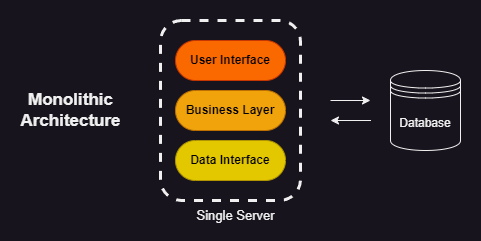
\includegraphics[scale=0.7]{monolithic_arch.png}
    \centering
    \caption{Monolithic Architecture}
    \label{fig:mono_arch}
\end{figure}

\section{Microservice Architecture}

Microservices and the Microservice Architecture have, in recent years, become one of the most popular design options for software applications. In the Microservice Architecture, the application is structured as a collection of independent services, called Microservices. Each Microservice corresponds to a distinct part of the business logic, executing a well-defined, unique process\cite{monovsmicro}\cite{microservicesdef}. These Microservices utilize lightweight communication mechanisms, such as API interfaces, allowing them to operate in unison and achieve the same final results as a Monolithic application but without being co-dependent. The independence of Microservices enables them to be built and tested separately, and they can be deployed and scaled independently as well. Each Microservice is designed to facilitate a single function of the application, making it focused, manageable, and easily comprehensible\cite{chandrinos_thesis}.

The advantages of this architectural approach compared to its Monolithic counterpart are significant and far-reaching. Each individual Microservice can be developed in isolation, often by different teams, without compromising or delaying the development of other parts of the application. This separation of concerns allows for parallel development, reducing bottlenecks and improving efficiency. Consequently, different components of the application can be updated and enhanced asynchronously, resulting in quicker and more frequent deployments. The build and deployment process is streamlined and resource-efficient since only the Microservice being updated needs to be redeployed, rather than the entire application.

Testing is another area where Microservice architecture shines. Since each Microservice operates independently, there is no need to build and test the entire application for changes made to one component. Instead, testing can be focused solely on the Microservice being modified. This leads to faster and more efficient testing cycles, allowing development teams to identify and resolve issues promptly. Similarly, debugging is simplified; when an error occurs, it is relatively easy to pinpoint the Microservice responsible for the failure. The responsible team can address the issue without disrupting the operation of the entire application, making the debugging process both quicker and more effective.

While these advantages are compelling, the most critical benefit of the Microservice Architecture is scalability. In the era of cloud-native applications, where the ability to scale up or down on demand is of utmost importance and operational costs are often usage-based, Microservice-based applications significantly outclass their Monolithic counterparts. Scaling in a Microservice application is versatile, as it is possible both vertically and horizontally. The entire application can be replicated if necessary, just like a Monolithic application. However, the true strength of Microservices lies in the ability to scale individual components. For example, if one Microservice experiences a spike in demand, only that specific service can be scaled up, optimizing resource usage.

Moreover, Microservice-based applications align seamlessly with cloud infrastructure. Since Microservices can be readily instantiated as needed, there is no requirement for maintaining multiple always-on instances to handle demand spikes, as is often the case with Monolithic applications. This elasticity in scaling reduces idle resource consumption and exponentially decreases operational costs.

Despite these numerous advantages, the Microservice architecture is not without its drawbacks. The initial development of Microservice applications requires careful and time-consuming planning and design. During the early stages of development, requirements and features are often not well defined, making it challenging to design Microservices effectively. Any missteps in the design can lead to significant complications later on.

Performance is another area where Microservice-based applications can fall short compared to Monolithic ones. Because Microservices rely on lightweight communication mechanisms, such as APIs, there is an inherent overhead in inter-service communication. This can result in latency, making Microservice applications less suitable for time-critical operations, such as load balancers or real-time data processing. For use cases requiring the lowest possible response times, Monolithic applications often have a performance edge.

Finally, Microservice architecture may not be the best choice for on-premises applications where customers are required to set up and manage everything manually. The complexity of configuring and maintaining multiple independent services can be overwhelming for end-users, especially those without extensive technical expertise. In such scenarios, a Monolithic application might be preferable due to its simplicity and ease of deployment\cite{whenmicroarebad}.

\begin{figure}[!h]
    \graphicspath{ {./diagrams/} }
    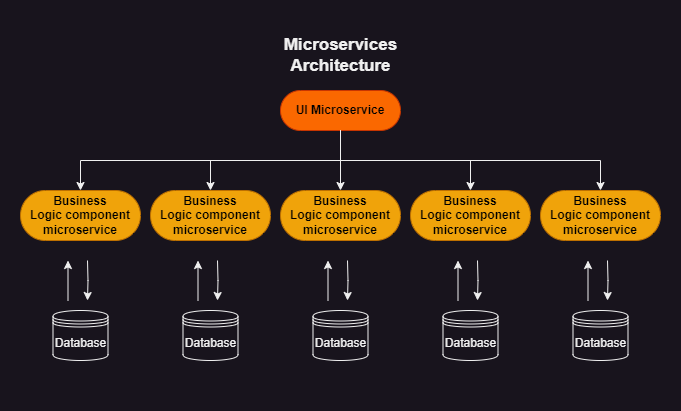
\includegraphics[scale=0.6]{microservice_arch.png}
    \centering
    \caption{Microservice Architecture}
    \label{fig:micro_arch}
\end{figure}

\section{Containers}

Hand in hand with the Microservice Architecture came containers. Containers are a form of virtualization similar to virtual machines (VMs), but unlike traditional virtual machines, containers share the host system's kernel while running in isolated user spaces. This architecture makes them significantly more lightweight, efficient, and versatile compared to VMs. By eliminating the need for a full guest operating system, containers reduce resource overhead dramatically, enabling more efficient utilization of host hardware. This efficiency translates to faster startup times, reduced memory and processing power requirements, and greater performance from the same hardware infrastructure compared to VMs\cite{Pahl2015}.

The lightweight nature of containers is particularly advantageous in scalable environments where applications need to scale up or down quickly in response to demand. In contrast, VMs require a separate guest operating system for each instance, which not only increases resource consumption but also lengthens deployment and startup times. Containers, on the other hand, are designed to spin up almost instantly, enabling rapid scaling and responsiveness.

Containers are created and deployed using container images, which are essentially templates. These images are built using ContainerFiles, which specify a base image and a sequence of instructions or steps to execute on top of it. Each step in the build process forms a new layer. Layering is a critical feature for image creation and deployment workflows, as it allows for reuse across different images. For instance, if multiple container images share common steps, such as installing a specific library, those layers need to be built only once. This reuse drastically reduces build times and conserves storage space, making containerization particularly well-suited to agile development practices where frequent builds and deployments are standard.

The distribution of container images is made straightforward through container registries, platforms where images can be stored, shared, and accessed. Docker Hub is the registry associated with the most popular container platform, Docker. The ability to easily distribute container images enhances collaboration and accelerates development cycles. Teams working in different environments can seamlessly pull images from registries, ensuring consistent runtime environments and reducing potential configuration mismatches.

One of the key strengths of containers lies in their ability to provide a consistent runtime environment. By encapsulating all dependencies and configurations within the container image, containers ensure that applications run identically across development, staging, and production environments. This consistency simplifies the testing and deployment process, minimizing release time and reducing the likelihood of environment-specific bugs.

However, as the use of containers grows, managing a large number of containers across multiple hosts becomes increasingly complex. Efficient deployment and management of containerized applications require some form of orchestration. Container orchestration platforms, such as Kubernetes, have emerged as the standard solution for automating the deployment, scaling, and management of containerized applications\cite{dockerDev}. Such platforms ensure high availability by intelligently distributing containers across nodes, maintaining desired states even during failures, and handling incident recovery automatically.

Moreover, they provide capabilities such as load balancing and resource allocation, enabling developers to build resilient and scalable systems with minimal manual intervention. Another major feature of these platforms are rolling updates, which ensure that new versions of an application can be deployed without downtime and handle rollback processes in case of failure. These features are only possible by taking advantage of the lightweight, lightning-fast deployment of containers and not only enhance the performance and reliability of applications but also reduce the operational burden on development teams.

\begin{figure}[!h]
    \graphicspath{ {./diagrams/} }
    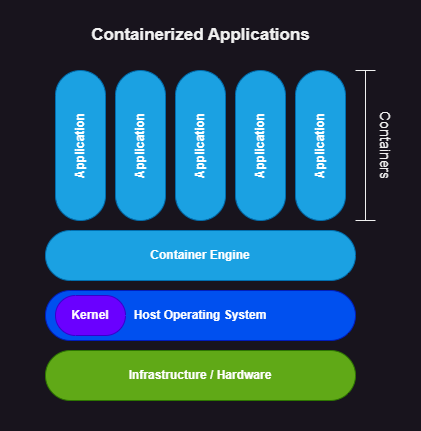
\includegraphics[scale=0.65]{containers_structure.png}
    \centering
    \caption{Containerized Applications}
    \label{fig:containerized_apps}
\end{figure}

\section{IoT device Simulators}

There's little doubt that the Internet of Things (IoT) is here to stay. IoT has reshaped the way humans and machines interact with the environment, creating smarter, more connected systems that are now strongly influencing most industries. In recent years, an increasing number of everyday devices have been equipped with various sensors and internet connectivity, enabling them to gather and transmit large volumes of data. This exponential growth of IoT devices has brought about significant opportunities, but it also presents unique challenges.

The data generated by IoT devices is massive and diverse, requiring robust IoT applications to process, analyze, and utilize it effectively. These applications are designed to transform raw data into valuable insights, enhancing the functionality of devices, and promoting efficiency in operations. However, as with any software, IoT applications must undergo rigorous testing before deployment to ensure reliability, security, and optimal performance.

One approach to testing IoT applications is to create a physical IoT network composed of the actual devices and sensors specific to the application. This setup allows for real-world data generation and provides an environment for testing the application under realistic conditions. While this method has its merits, it is not hard to notice the significant challenges and limitations it poses.

First and foremost, creating an actual IoT network for testing can be prohibitively expensive. IoT ecosystems often consist of diverse and specialized devices, many of which may be costly to acquire or replicate at scale. For large and complex ecosystems, the financial overhead of assembling and maintaining such a network can be quite substantial, making this approach impractical in most cases.

Furthermore, IoT applications, particularly in the early stages of development, are subject to frequent redesigns and changes. These iterations are part of the development process as requirements change, features are added, and feedback is provided. However, when an IoT network is used for testing, any significant change in the application may necessitate corresponding changes to the physical network. This adds to the development cost and introduces delays, as modifying or expanding an IoT network is both time-consuming and resource-intensive.

Even when an IoT network is already in place for deployment purposes, using it for application testing poses additional risks. Testing on a live network can expose sensitive data to potential security vulnerabilities.

To address these challenges, a more efficient and safer alternative is the use of synthetic data. Synthetic data simulates the behavior and output of real IoT devices, providing a realistic representation of IoT network activity without requiring a physical network. This approach allows developers to create virtual IoT environments tailored to specific applications, enabling thorough testing under controlled conditions.

By generating synthetic data, developers can replicate complex IoT ecosystems at a minimum cost compared with physical networks. These virtual environments can be easily modified to accommodate changes in the application, supporting agile development without the need for expensive hardware adjustments. Additionally, synthetic data eliminates the security risks associated with using real-world data during testing, as no actual devices or sensitive information are involved.



\begin{figure}[!h]
    \graphicspath{ {./diagrams/} }
    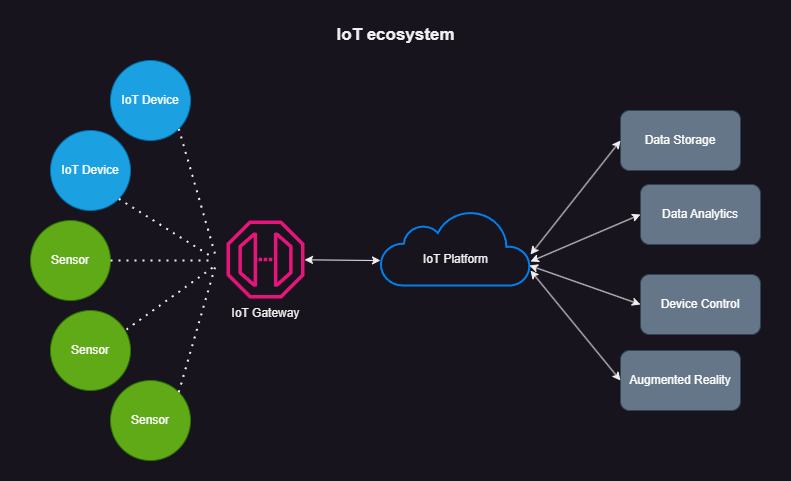
\includegraphics[scale=0.55]{iot.png}
    \centering
    \caption{IoT ecosystem}
    \label{fig:iot_eco}
\end{figure}